% Chapter 1

% variables
\newcommand{\pdirone}{chapters/plots/chapter1}

% cross references

\chapter{Why Dark Matter?} % Main chapter title
% \chapter{Introduction} % Main chapter title

\label{chapter1}

In this first chapter, the concept of Dark Matter and its history will be introduced. In Sec.\ref{ch1:sec:dm-evidence} we will explore why we need this concept, and what are the alternatives to it. After that, we will come to realize that Dark Matter is a very simplistic term, that hides an extremely large number of possibilities that can be constructed using the framework of Quantum Field Theory (QFT). Dark Matter candidates are indeed very numerous, but we can focus on the most reasonable ones, that do not require very complicated models. In Sec.\ref{ch1:sec:dm-candidates} we will give a small review on these possibilities. The main focus of my thesis will be the so-called Dark Sector, where Dark Matter particles can interact with the Standard Model using new undiscovered interactions. The vector portal will be introduced, which postulates the existence of an additional $\textrm{U(1)}$ symmetry that generates a "Dark Sector" of particles amounting to the invisible matter. The vector gauge boson generated by this symmetry, that we will label $\DM$ through this thesis, has been known with the catchy name of Dark Photon, due to playing the equivalent role of the standard model photon in this new symmetry. This model allows also a cross-term that couples the new Dark Photon with its standard counterpart, effectively building a portal between the two sectors. If such a model is true, we can produce this type of matter using modern accelerators, allowing us to perform a particle physics experiment to probe this model. After this introduction, we will see how Dark Matter can be searched using particle beams in the context of fixed-target experiment. Starting from the benchmark model $\umodel$, the signal yield expected in such experiments is derived for different decay modes. The production of Dark mediators in colliders is not limited however to vector bosons only, but can be extended to a large group of models that predicts small interactions between the Dark Sector and particles from the standard models. Some of these additional searches, like the one for axion and axion-like scalar mediators, were already performed by the NA64 .
% But why this model should be better than the others? There is not an easy answer to this. From a scientific point of view, a model is better than another if it is more powerful in explaining the data collected. However, sometimes a model can solve more than one problem at the same time, which makes it especially attractive for scientists. Originally, the Dark Photon was also an excellent explanation of the measured value of the anomalous muon magnetic moment, that to date deviates substantially (by $\sim$3.6$\sigma$) from the prediction of QED. We now know that such an explanation is ruled out since NA64 together with other experiments excluded it.
Another phenomenon that could be explained in this framework is the so-called $\DMX$-anomaly, originally known with the name of $^8$Be-anomaly. This name refers to a bump detected in the nuclear decay spectrum of Beryllium that would be justified by the existence of a particle not present in the standard model. In Sec.\ref{ch1:sec:dm-u1model-motivations-x17} a review of this phenomena will be given, and we will show how particle physics explanation of this anomaly are within the sensitivity range of the NA64 experiment.

%----------------------------------------------------------------------------------------

\section{Evidence for Dark Matter}
\label{ch1:sec:dm-evidence}

The story of Dark Matter and the birth of this term is interesting on its own, and a good example of "unequivocal accumulated evidence" in science, but in a way is even more than that \cite{hooper, deSwart:2017heh}. The term was first used in 1937 by astronomer Fritz Zwicky\footnote{Some weaker claim of a discrepancy was observed even before by Knut Lundmark in 1930.} to justify the velocity dispersion in Coma cluster galaxies, which were deviated significantly from what predicted by simply asserting the mass from the visible matter. This hypothesis was discussed more seriously in 1950 when astronomical surveys confirmed these results with high precision. This sparked a heated debate in the scientific community, and many solutions to this problem did not include additional unknown matter, but rather the modification of gravity or more sophisticated arguments based on the dynamical equilibrium of such galaxies. In 1970 with the rising of radio astronomy the rotation curved of galaxies are studied in detail, and two studies performed by Kenneth Freeman and Vera Rubin separately confirm that the velocity of rotation of objects in a galaxy becomes flat at sufficient distance from its center. The idea becomes very influential to the cosmological community thanks to two papers in 1974 by Einasto and Ostriker, clearly stating that the mass of galaxies has been underestimated by a factor 10 until then \cite{EINASTO1974,1974ApJ...193L...1O}. This was further strengthened by the end of the decade by very similar analysis, summarized in this review \cite{annurev.aa.17.090179.001031}. The existence of Dark Matter becomes more and more accepted in the years to come, alternative theories also arise to explain observation without the need of additional matter. Perhaps the most famous today remains the MOND theory, built as a weak-field approximation of some more general theory of gravity yet to be discovered. Despite some early success, this theory has always proven to be challenging to merge in the general relativity framework, and is insufficient to justify some specific phenomena like the famous "bullet cluster", that is on the other hand very well explain by Dark Matter \cite{Clowe_2006}.

So what is the current situation of Dark Matter? Today the theory is well accepted in the scientific community, although some debate is still present. The existence of Dark Matter is the leading paradigm to explain all discrepancies observed \cite{hooper}. Advances in the field of cosmology and measurements technique have provided much other evidence that aid Dark Matter existence. For example, gravitational lensing, in particular in the context of weak lensing, was used to characterize the mean distribution of Dark Matter and match it to the one predicted by large scale structure measurements \cite{weak-lensing}. Temperature anisotropies of the Cosmological Microwave Background (CMB) also present structures compatible with Dark Matter, and well fitted in the $\Lambda$CDM model\footnote{More detail on this model are provided in Appendix.\ref{AppendixA}} \cite{Ade:2015xua}. Many other arguments, including structure formation \cite{Navarro:1995iw}, baryon acoustic oscillation \cite{bao}, and Red-shift distortions \cite{Peacock2001} have proven consistently to agree with Dark Matter existence and with the $\Lambda$CDM model in particular.

While the consensus on its existence is well established in the scientific community, its origin and exact composition is a big mystery still today. In the next section, we will try to give an overview of what exactly defines Dark Matter, starting from its measured properties. After that, we will explore the most popular models that try to explain this puzzle.
%So let us assume like the majority of the scientific community that Dark Matter indeed exists, what is its exact nature? Can we point down some characteristics and a space of parameter that defines it exactly? Those are the questions that will be answered in the next section.

\section{Dark Matter candidates}
\label{ch1:sec:dm-candidates}

The first to ask ourselves is what kind of property Dark Matter should have to satisfy the experimental constraint given by cosmology. We can define the following key characteristics \cite{Profumo:2019ujg}:

\begin{itemize}
\item \textit{Dark}: It should not emit light, but a tiny charge is still compatible with data, which justifies models with "milli-charged" particles. What is effectively constraint is the ratio of charge to a power of the mass.
\item \textit{Collisionless}: Dark Matter self-interaction to mass ratio is constraint by observation of cluster mergers and the ellipticity of galactic halos. The cross-section itself is not however necessarily small, assuming a mass similar to the one of a proton. The constraint amount to a cross-section in the order of barn, very similar to the one observed for the strong interaction.
\item \textit{Classical}: Dark Matter is observed to be confined on the galactic scales of a few kpc in dwarf galaxies. Hence, their de Broglie length must be smaller than that to have a coherent Dark Matter halo. This argument is typically used to put a lower limit on the DM mass. If the Dark Matter candidates is a fermion, constraints are stronger as Pauli blocking limits the density to at most the phase space density to $f=gh^{-3}$ where g is the number of internal degrees of freedom.
\item \textit{Fluid}: For macroscopic DM, with a mass much larger than the solar mass $M_{\odot}$, tidal disruption is expected to break the stability in a globular cluster. This limit is typically placed around $10^6 M_{\odot}$.
\end{itemize}

In summary, while the cosmological and Galactic Dark Matter density is known to a good degree, very weak constraint exists on the interaction strength and the exact mass of Dark Matter. The huge mass scale that spans over the possible region is depicted in Fig.\ref{fig:dm-mass-range}, where we see several possible DM candidates in relation to their possible mass and search technique to probe them. A few experimental anomalies are labeled in red to see mismatches between theory and experiment that could potentially be explained by Dark Matter. We can see that most of them are in the \mev-\gev scale, which is the one covered by our experiment. Even the problem of the cosmological scale, like small-scale structure, are potentially well explained by this class of models \cite{battaglieri2017cosmic}.

\begin{figure}[bht!]
  \centering
  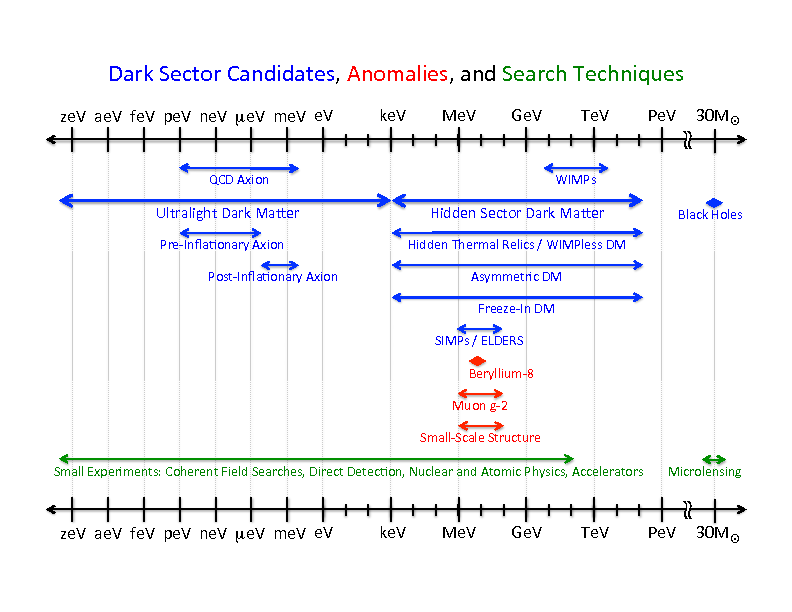
\includegraphics[width=\textwidth]{\pdirone/DM_summary.pdf}
  \caption[Mass range for Dark Matter]{Mass range for Dark Matter and mediator particle candidates, experimental anomalies, and search techniques.}
  \label{fig:dm-mass-range}
\end{figure}

Because of the relatively loose constraint, it comes to no surprise that a vast amount of models have been theorized for the explanation of DM. The ones depicted in Fig.\ref{fig:dm-mass-range} are only a subset of what is possible. Some models can be extended to be explained in scales not included in their original incarnation. It is the case for Axion Like Particles (ALPs), that are an extension of the QCD Axion model originally developed to solve strong CP problem \cite{PhysRevD.16.1791}. Contrary to Axions, their mass $m_a$ is taken as an independent parameter from their main coupling $g_{a \gamma \gamma}$, and can be arbitrarily large. Indeed this mass can also be in the \mev-\gev scale, in the range where the NA64 experiment is sensitive. As we will show in Sec.\ref{ch4:sec:exclusion limits}, we already used our data to constraint a portion of this parameter space \cite{Banerjee:2020fue}.

Each single model of DM is out of the scope of this thesis. For a complete review, one can look at \cite{battaglieri2017cosmic,Profumo:2019ujg,HAMBYE2020135553,alex2016dark,review-particle-physics,Feng:2010gw}. Here, we provide a short description of the mainstream possibilities currently considered for Dark Matter:
\begin{itemize}
\item \textbf{\textit{WIMP}}: For a long time, Weakly Interacting Massive Particles (WIMP) were considered the most probable candidate by the scientific community. Their main characteristic is tree-level interaction with the W and Z boson, but not with gluons or photons. Historically, their mass is in the 10 \gev-\si{\tera\electronvolt}, although more recent models extended the mass range to lower masses as well. The so-called WIMP miracle \cite{Chang:2013oia}, provided a very effective and natural way to introduce Dark Matter in the thermal history of the early universe in a way that predicted precisely the current relic density. However, after an extensive amount of research, accelerators and direct search have to this date failed to provide evidence to their existence \cite{Arcadi:2017kky}. These models have yet to be ruled out completely, and remain to this date the most studied type of Dark Matter.
\item \textbf{\textit{Axions and Axion-like}}: Axion and Axion-like particles are obtained by introducing a new pseudoscalar field $a$ with coupling to photons \cite{Marsh:2015xka}. Originally Axions were motivated by the strong CP problem and they were predicted to be extremely light ($<$\si{electronvolt}). The model was later extended to offer a possible explanation for Dark Matter at higher masses. Several experiments based on the "light shining through a wall" concept or using a magnetic helioscope \cite{annurev.nucl.56.080805.140513} already put some stringent limits on Axions. Axion-like particles on the other hand can have a mass large enough to allow testing using accelerators.
\item \textbf{\textit{Sterile Neutrino}}: While Standard model neutrinos are not a good fit to explain Dark Matter as they are produced very hot in the early thermal bath, Sterile neutrinos are on the other hand a viable explanation and can be probed in direct detection experiments. A subset of these models can also explain the light neutrinos masses as a consequence of the \textit{see-saw} mechanism, although they are not favored as Dark Matter explanation \cite{Feng:2010gw}. 
\item \textbf{\textit{Dark Sector}}: By the name of Dark Sector, we describe a very large class of models characterized by particles not charged directly under strong, weak, or electromagnetic force \cite{alex2016dark}. Particles can still interact with the SM particle through additional interactions constraint by the symmetry of the standard model, called "portals" interactions. This class of models, specifically the ones charged under a new U'(1) symmetry, are the focus of the NA64 experiment, and they will be described in more detail in the next sections.
\end{itemize}

\section{The Dark Sector}
\label{ch1:sec:dm-sector}

Dark sectors , introduced in Sec.\ref{ch1:sec:dm-candidates}, are very interesting candidates to explain the origin of Dark Matter (see \cite{battaglieri2017cosmic,alex2016dark} for recent reviews). On the top of reproducing the observed DM abundance in freeze-out or freeze-in scenarios, many experimental anomalies currently observed can be explained inside this framework. The anomalous magnetic moment of the muon \cite{blum2013muon}, the proton charge radius \cite{Pohl2010} and more recently the $\DMX$-anomaly \cite{Krasznahorkay:2015iga,Krasznahorkay:2019lyl} have been suggested as possible hints of a dark sector \cite{alex2016dark}. The definition of this sector is extremely broad, and can accommodate many different models. Its physics however, can be explored effectively and in a systematic way by using specific portal interaction as classification scheme.  The existence of a mediator acting as a portal is a necessity to create a Dark Sector, but a small interaction with SM allows a signature in particle physics experiments as well as a mechanism to compute the observed relic density \cite{prw, pospelov}. The gauge and Lorentz symmetries restricts the ways in which the mediator can couple to SM particles. We can classify them using their spin and parity, and by excluding dimension operators larger than 5 we obtain four renormalizable possibilities \cite{alex2016dark}:

\begin{equation}
  \label{eq:dm-portals}
  \mathcal{L} \quad \supset \quad
\begin{aligned}
  &-\frac{\epsilon}{2 \cos{\theta_W}}B_{\mu \nu}F'^{\mu \nu}, &\textrm{vector portal}\\
  & (\mu \phi + \lambda \phi^2)H^{\dagger}H, &\textrm{Higgs portal}\\
  &y_n LHN, &\textrm{neutrino portal} \\
  &\frac{a}{f_a} F_{\mu \nu} F^{\mu \nu}, &\textrm{axion portal}
\end{aligned}
\end{equation}

In this work, we will limit the discussion on the vector portal, as it is the most viable for thermal models of LDM. If we assume the DM mediator to be a vector boson arising from an additional U'(1) gauge group under which the LDM is charged, we can derive a term $\epsilon / \cos{\theta_W} B^{\mu \nu} F'{\mu \nu}/2$ that is invariant both on this symmetry and the well known U(1) from QED. This can be used to explain the phenomenology of a large class of models, such as scenarios where the Dark Photon couples preferentially to Baryonic, leptonic, or (B - L) currents. One such case, where the coupling to Baryon is disfavored, is the protophobic $\DMX$ gauge boson \cite{PhysRevD.95.035017}, that will be introduced at the end of this chapter. Other possibilities includes the DM possessing a Majorana coupling to the mediator \cite{PhysRevD.93.063523}, or the existence of a rich sector \cite{Morrissey_2014}.

\subsection{The vector portal}
\label{ch1:sec:dm-colliders}

To discuss about the experimental implications of the vector portal, we need to establish a production mechanism that can be used to detect DM in an experiment. We start by building a vector portal introducing an additional $\umodel$ symmetry to the standard model lagrangian:
\begin{equation}
  \label{eq:dm-lagrangian}
  \mathcal{L}_{DS} = \mathcal{L}_{SM} \underbrace{- \frac{1}{4}F'_{\mu \nu}F'^{\mu \nu} + \frac{m_{\DM}}{2}A'_{\mu}A'^{\mu}}_{\textrm{U'(1)}} + \underbrace{i \bar{\chi} \partial_{\mu} \chi - m_{\chi}\bar{\chi}\chi - e_D \bar{\chi}\gamma^{\mu}A'_{\mu}\chi}_{\textrm{Dirac spinor}}
\end{equation}
This new symmetry introduced an additional gauge vector boson, called "Dark Photon" due to its equivalent role in the Dark Sector as the well known photon. In this work, we will label it $\DM$\footnote{The field will be labeled in the same way for commodity.}. Here we also added a Dirac spinor field $\chi$ that is coupled to $\DM$ by a coupling constant $g_D$. This is for the completeness of the model, which is also supposed to contain an LDM that justifies the relic density. There are however other possibilities to a simple Dirac fermion. The part of the lagrangian over the first parenthesis is the one generated by the new U'(1) symmetry and is the most relevant to compute the physics of the portal. In particular, the terms multiplied by $\epsilon$ represent the kinetic mixing between $\gamma$ and $\DM$, as it multiplies the two field tensor generated by the two U(1) groups. Here $\epsilon$ is taken as an a priori parameter that controls the strength of the kinetic mixing. it can in principle have any value, but being naturally generated inside loops of heavy fields charged under both symmetries, it is expected to be small, in the range $\epsilon \sim 10^{-8} - 10^{-2}$ \cite{jdb}. 

The channels that allow the production of this new boson $\DM$ are similar to the one that can be used for $\gamma$ as they both are the generators of a U(1) symmetry. In first order they are the following:

\begin{itemize}
\item \textit{Dark Bremsstrahlung}: The reaction $\darkbrem$ where $\DM$ is emitted after a virtual photon is exchanged with a target nucleus.
\item \textit{Dark Compton}: The reaction $\darkcompton$, where $\DM$ is produced as a consequence of the interaction of a photon and an electron.
\item \textit{Dark Resonance}: The reaction $\darkresonance$ where two leptons annihilated and produce an $\DM$ as a consequence of a resonance.
\end{itemize}

The Feynman diagrams of all processes mentioned above are depicted in Fig.\ref{fig:dm-production-mechanism}.

\begin{figure}
\centering
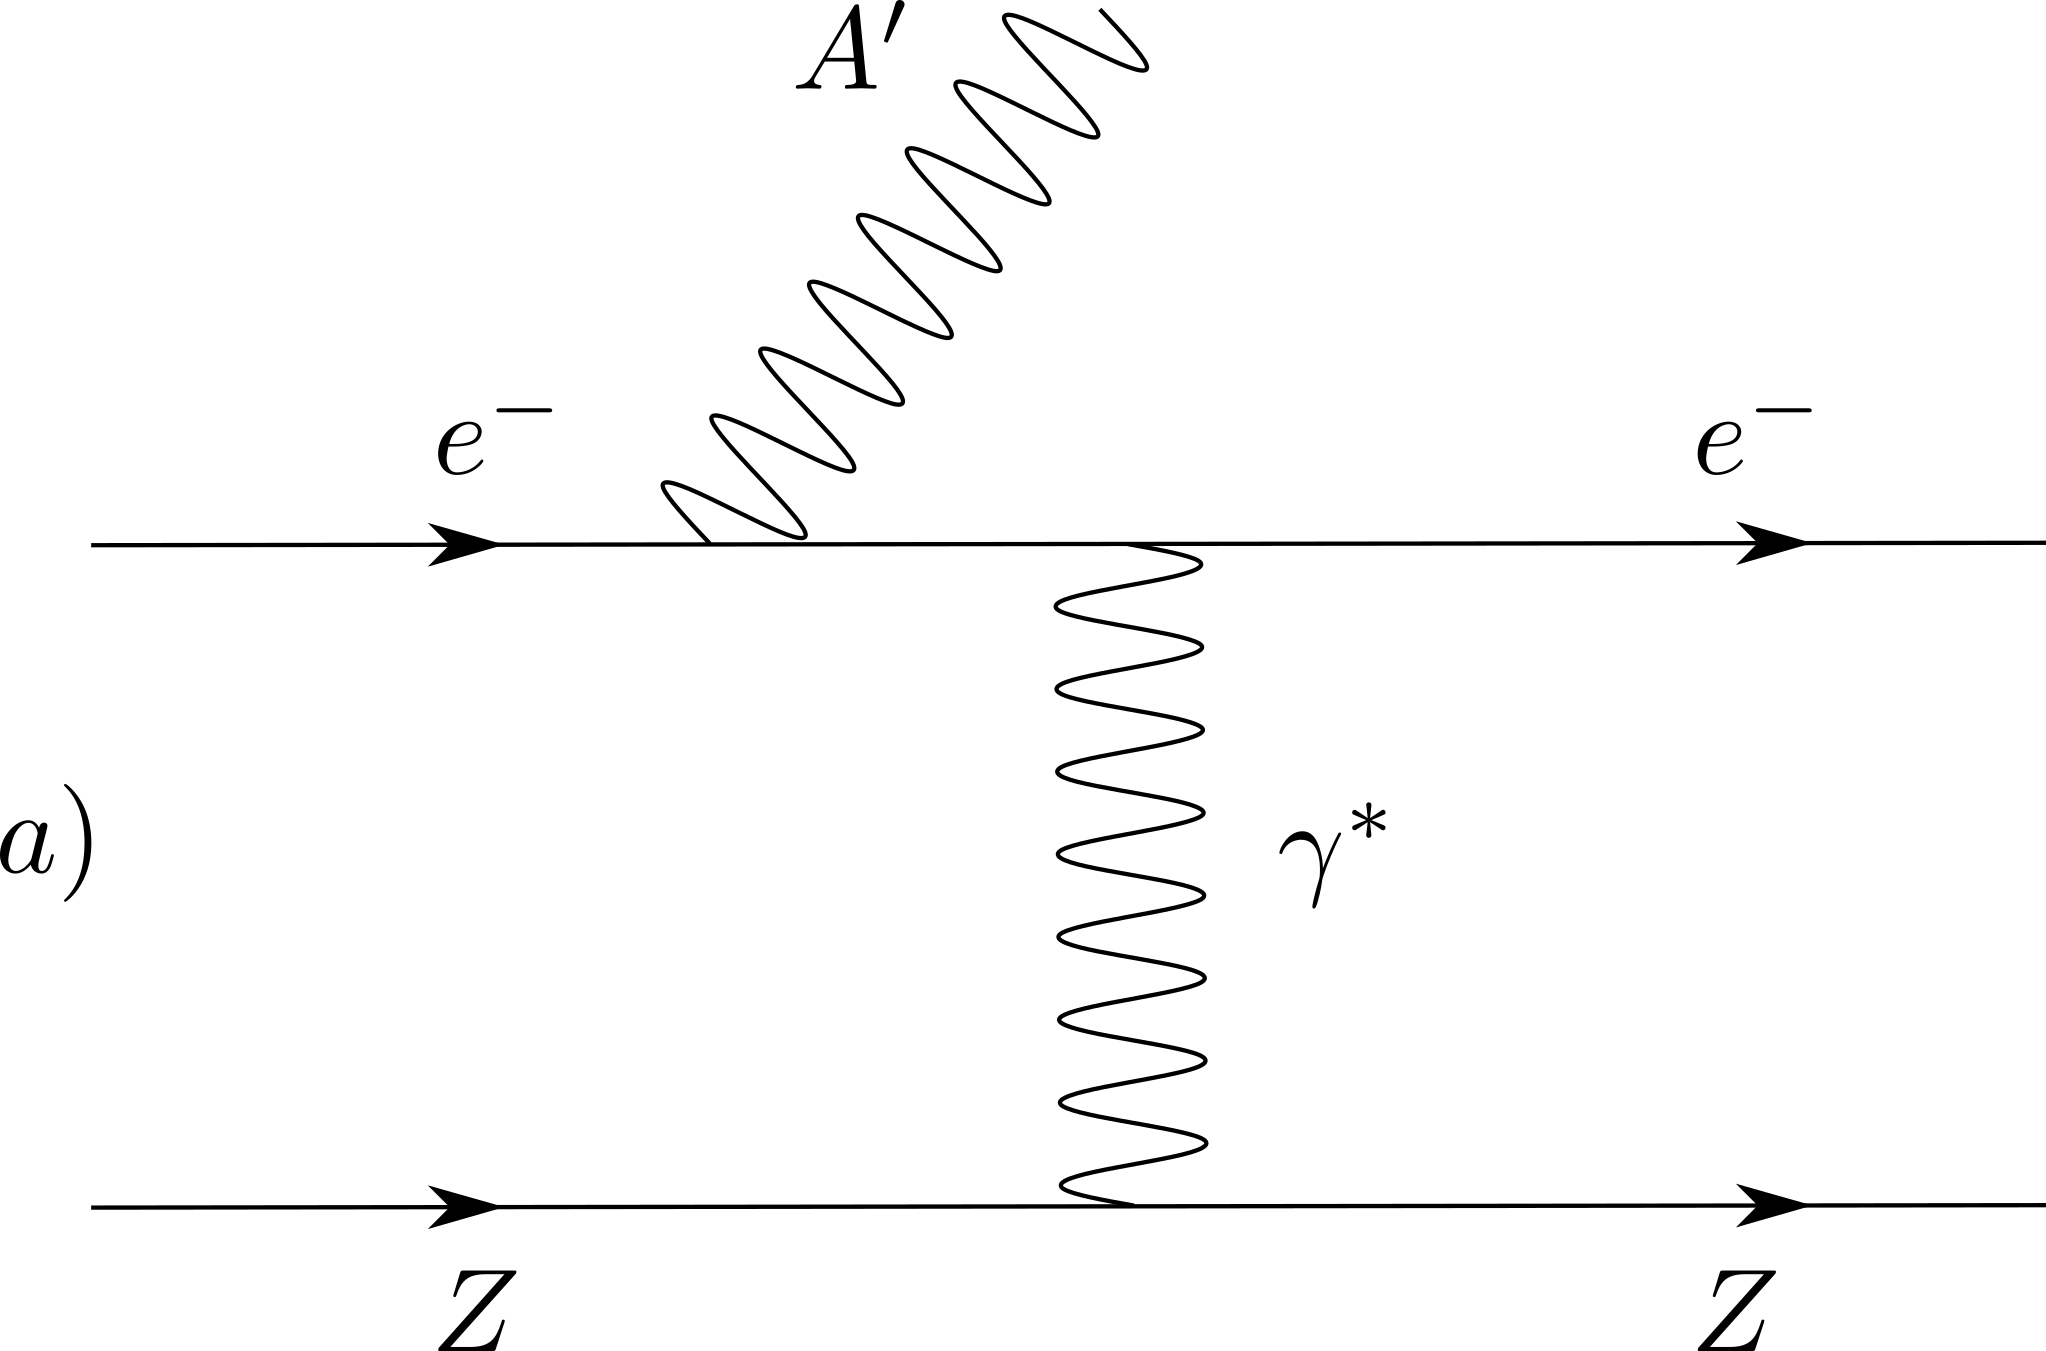
\includegraphics[width=.45\textwidth]{\pdirone/DarkBremstrahlung.png}
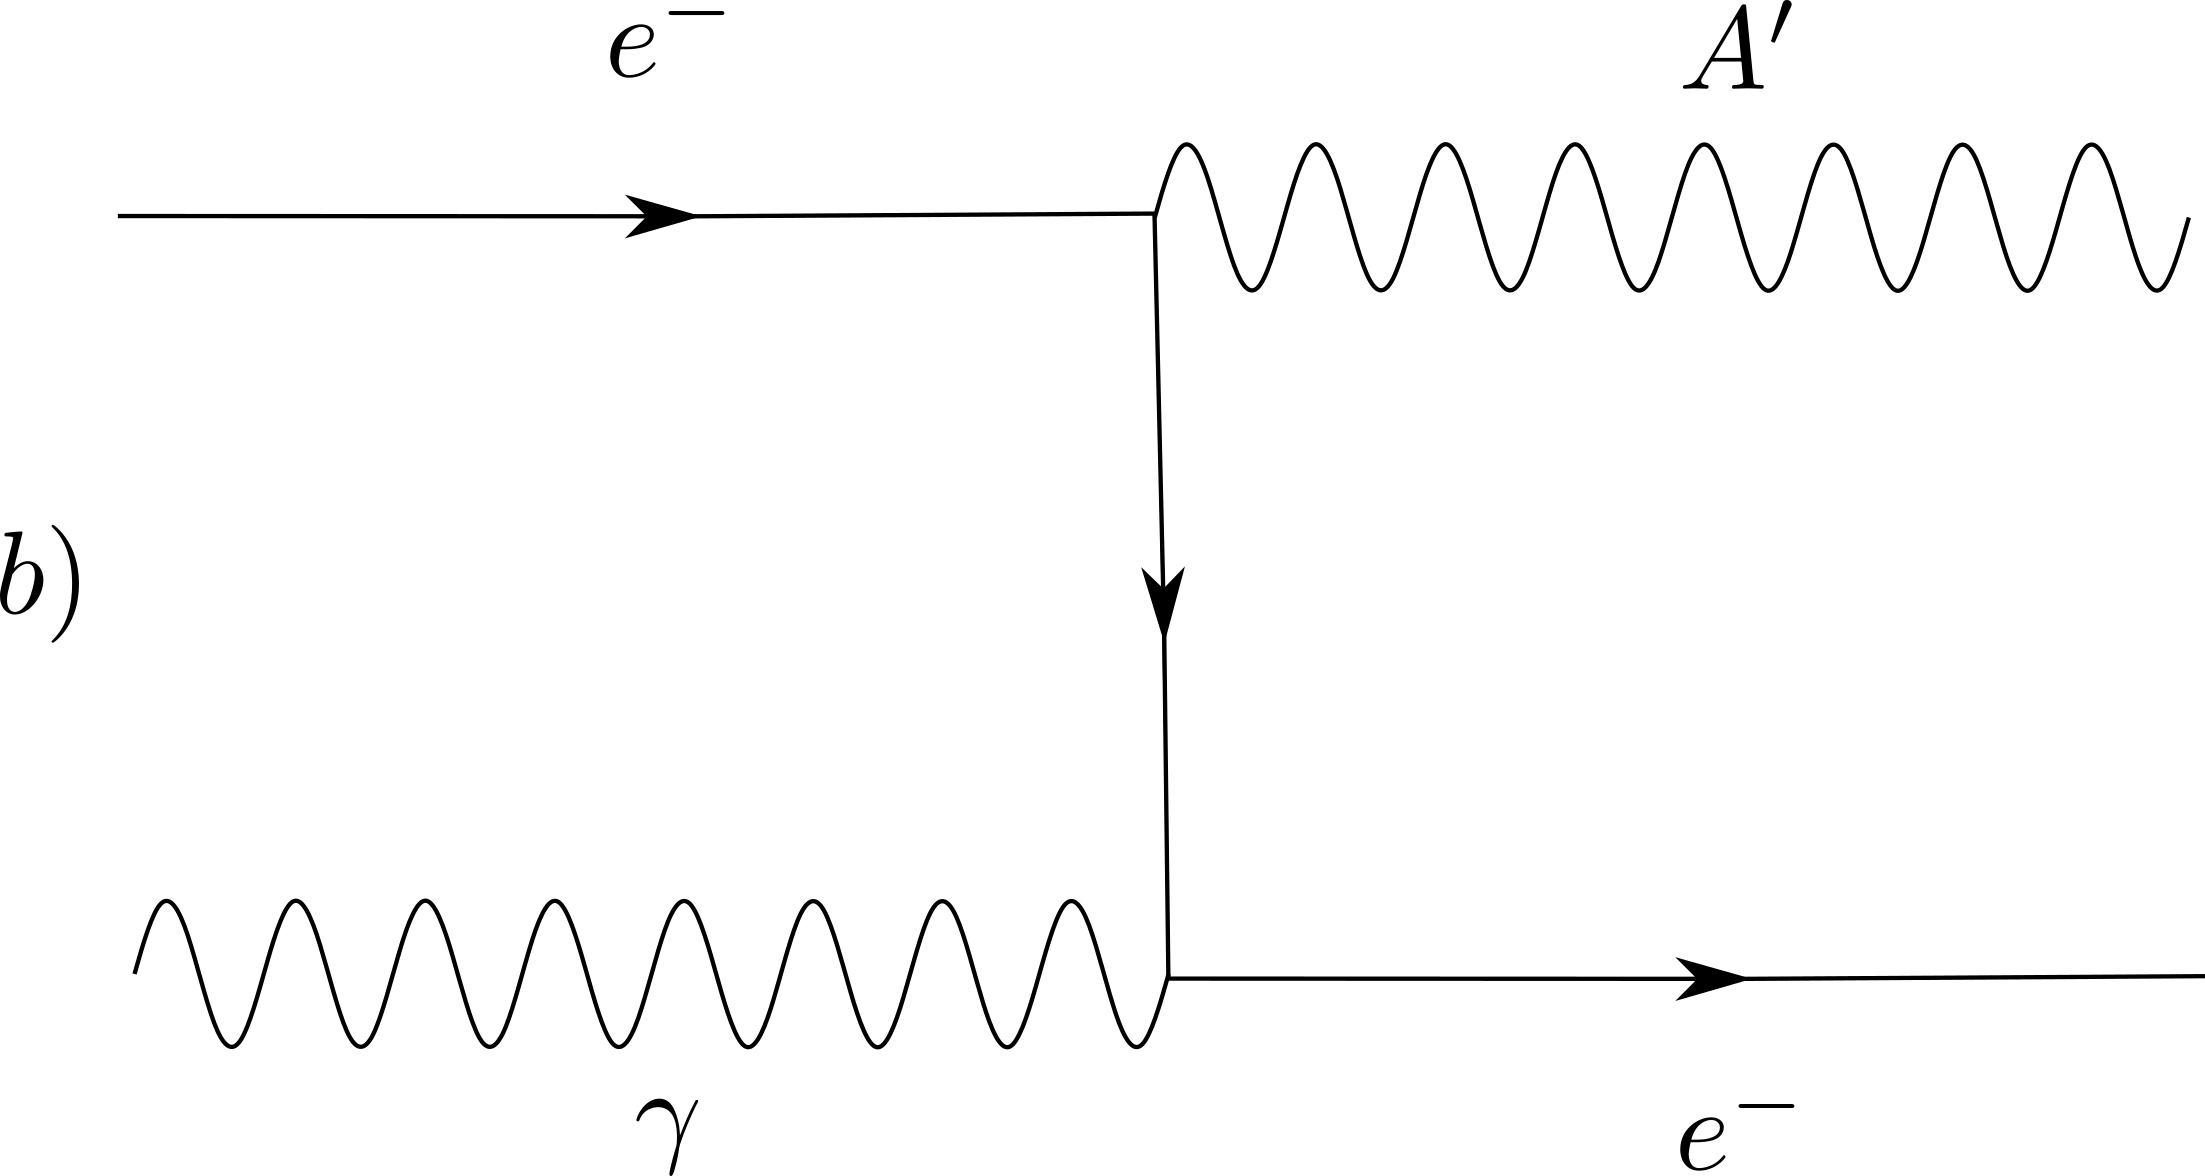
\includegraphics[width=.45\textwidth]{\pdirone/DarkCompton.png}
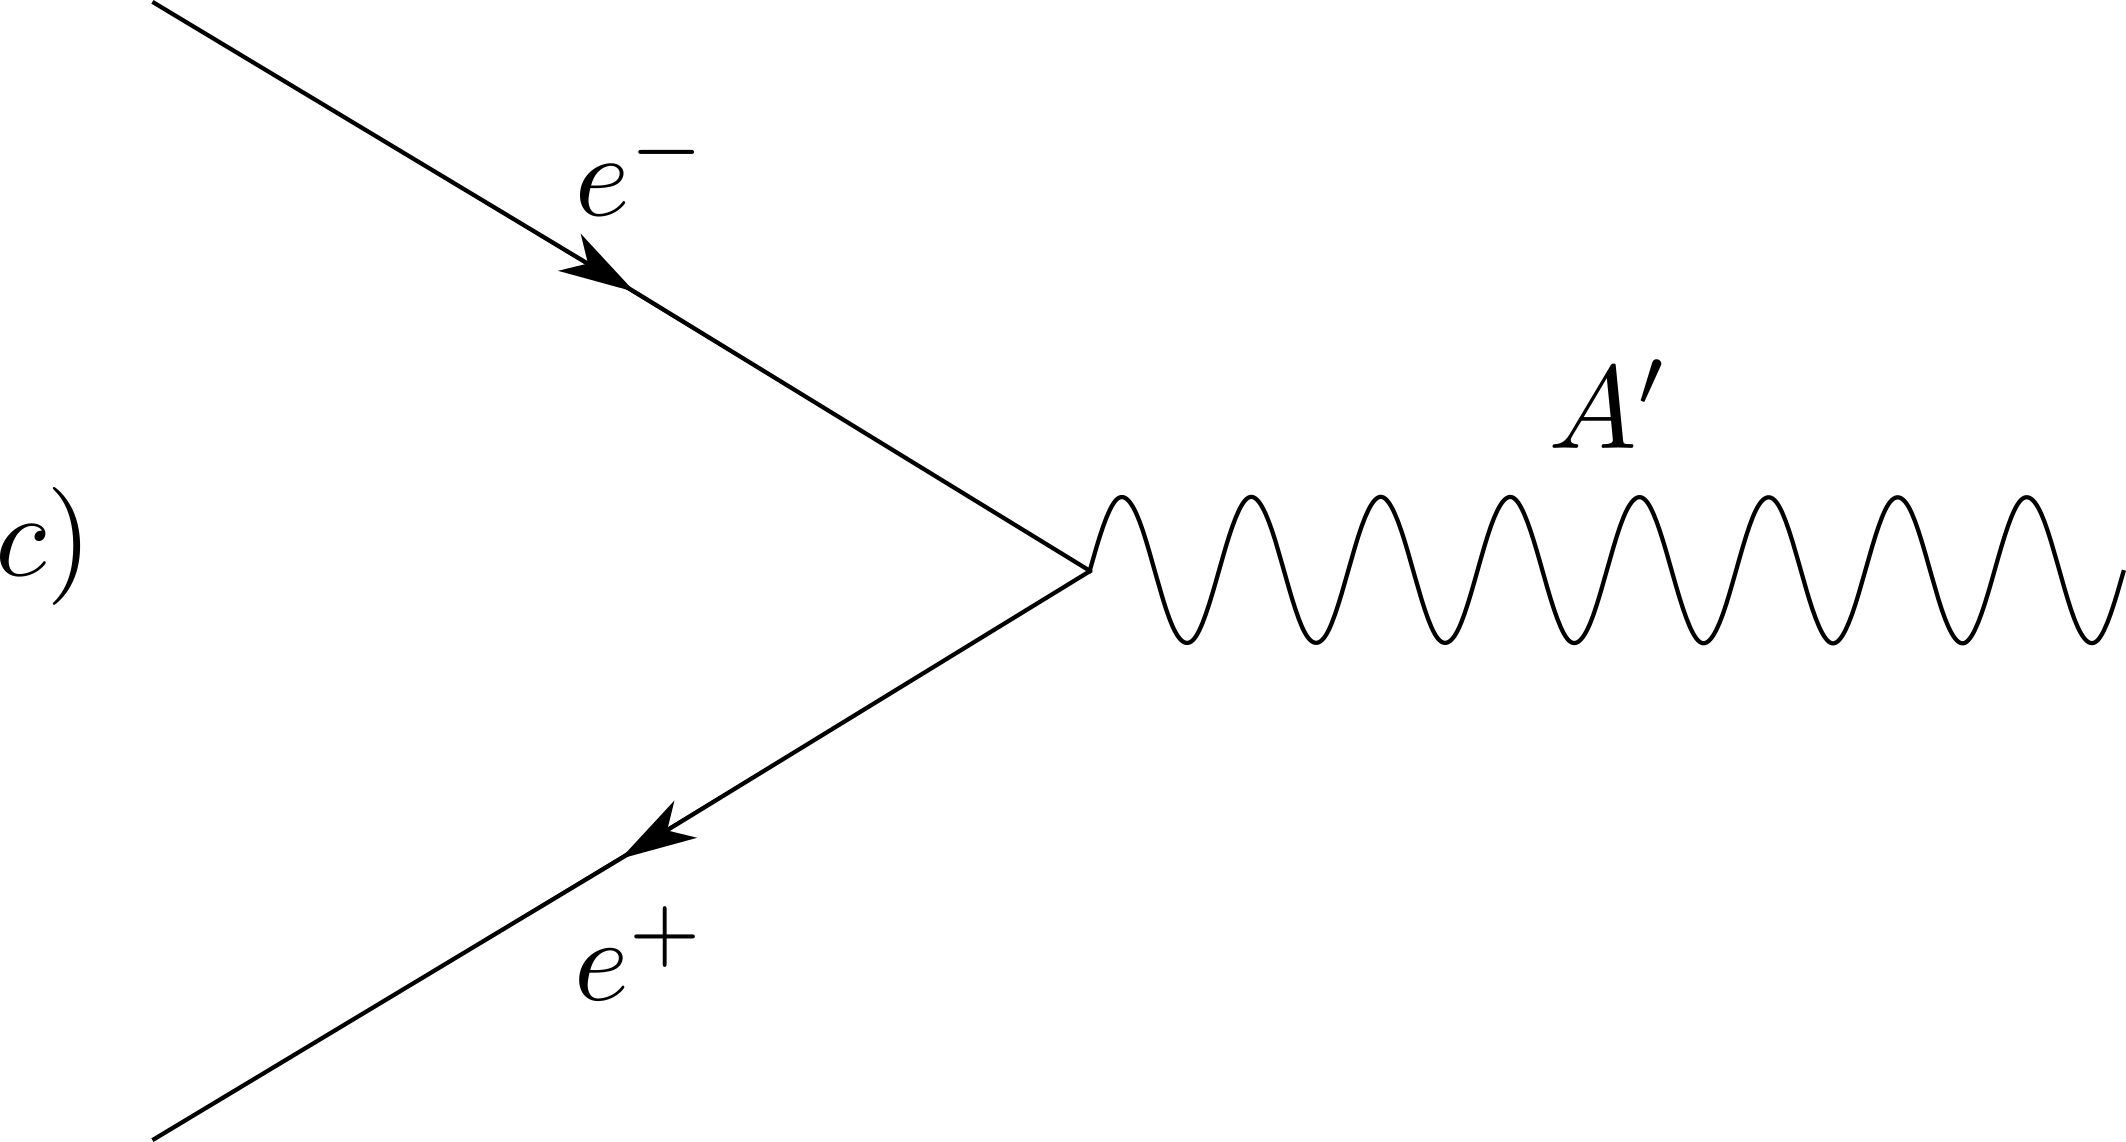
\includegraphics[width=.45\textwidth]{\pdirone/DarkResonance.png}
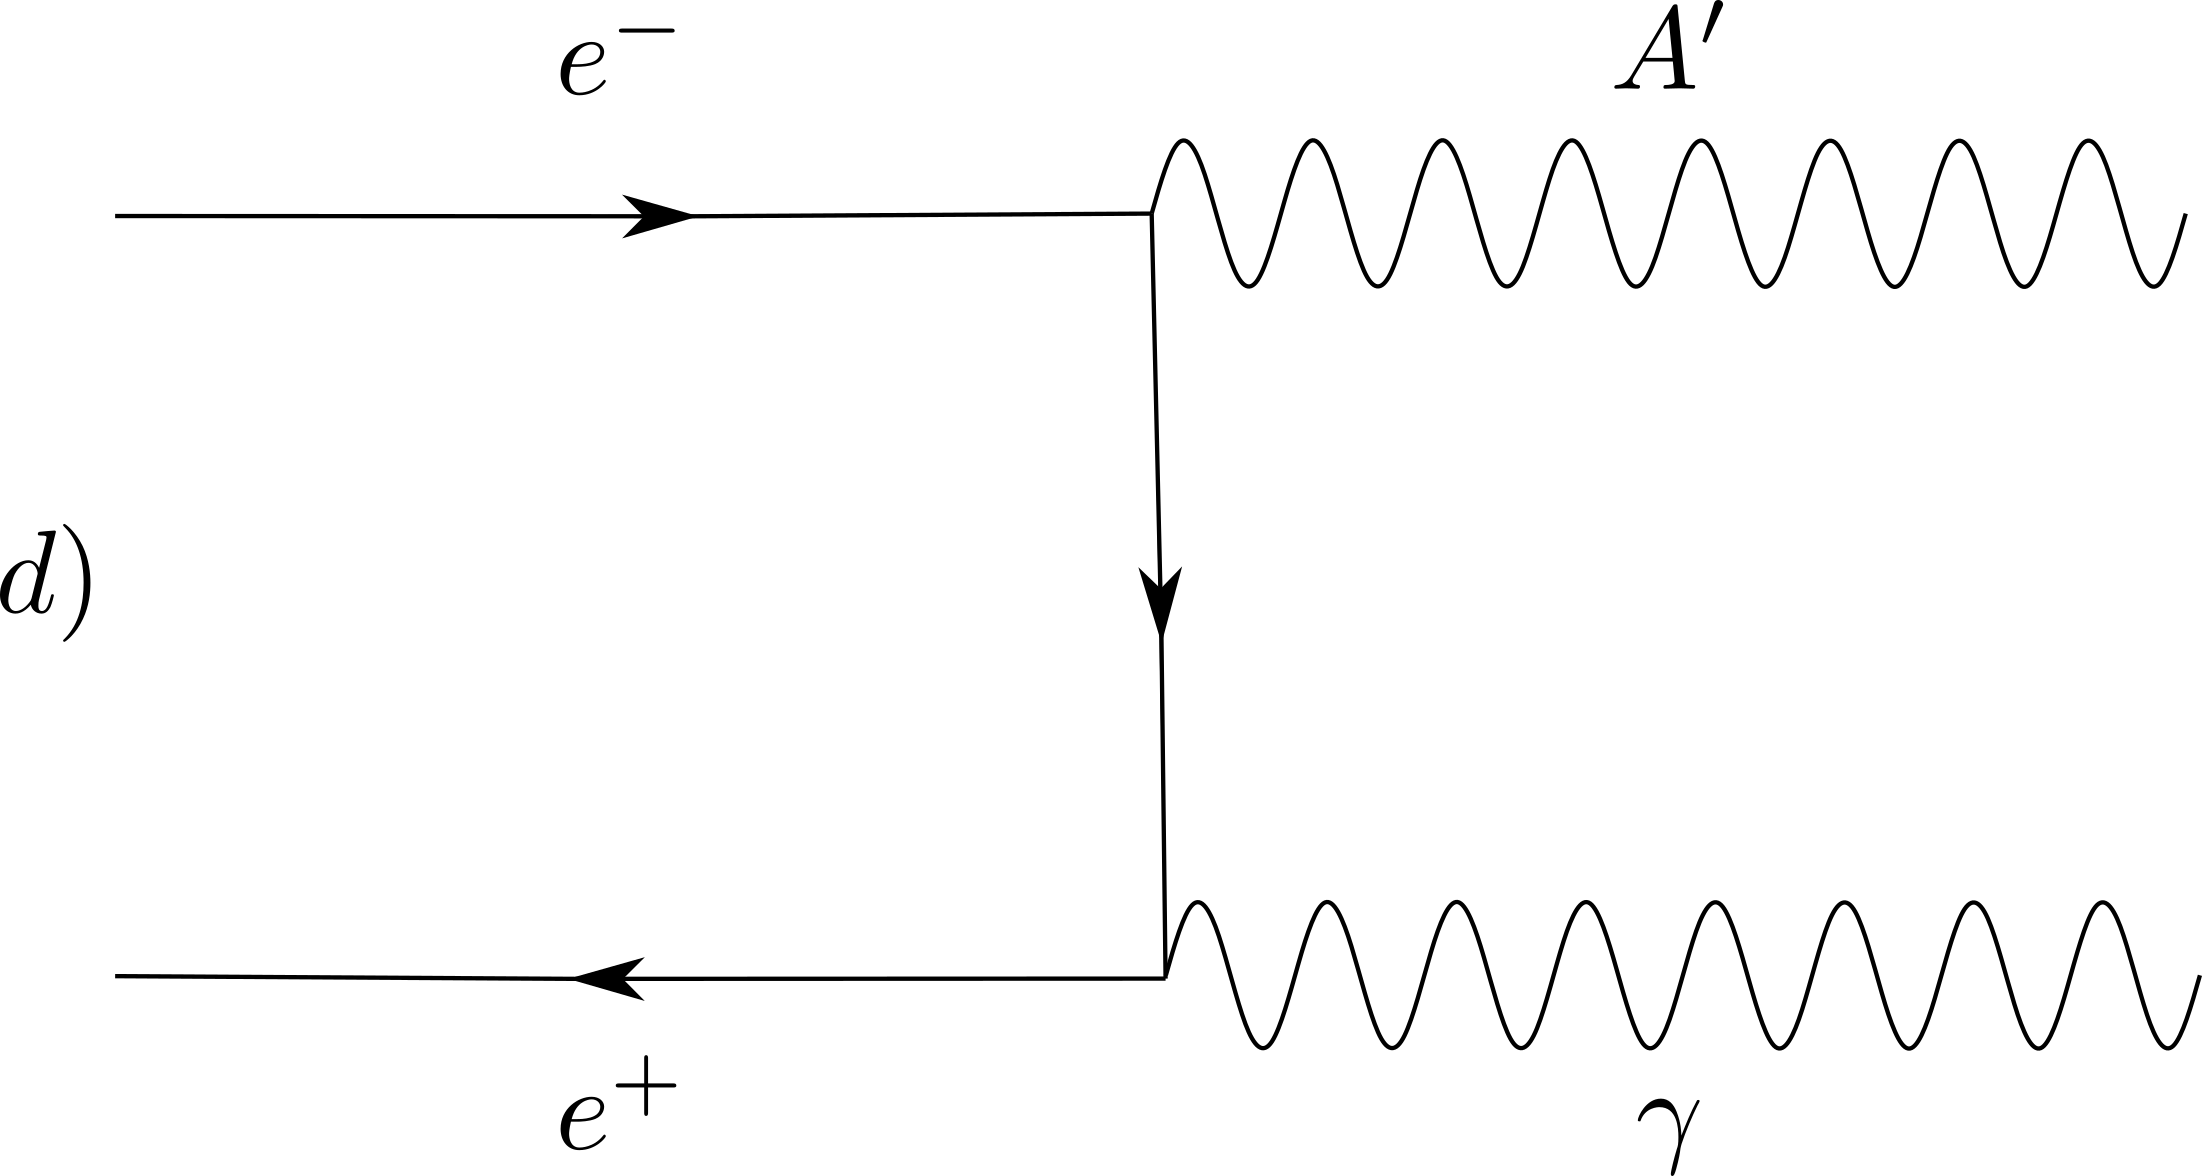
\includegraphics[width=.45\textwidth]{\pdirone/DarkAresonance.png}
\caption{Possible production mechanism for $\DM$: Dark Bremsstrahlung a), Dark Compton b), resonance production c) and A-resonant production d).}
\label{fig:dm-production-mechanism}
\end{figure}

Other channels might be possible with minimal extension of the model, or one could find a significant yield of production not only in the scattering of an electron but also using another type of primary. An example would be using the electromagnetic portion of a large hadron shower to compute the yield of $\DM$, which was suggested as possible future method to search for low mass $\DM$ in \cite{Celentano:2020vtu}.

When a high energy particle hits a thick target, all of the mentioned mechanism will be relevant to some degree. %One might object that the particles needed for each production channel are different. Indeed while a nuclei Z is always present in matter, the presence of a $\gamma$ or a $e^+$ might not be as straightforward if one starts for example from an electron beam. In an electromagnetic shower originated by a high energetic lepton, however, all three particles will be produced in large quantity due to the subsequent process of pair-production and Bremsstrahlung that are the most relevant for high energetic $\gamma$ and high energetic $\ee$ respectively \cite{Bichsel:2002cf}.
In most fixed-target experiments, however, the Dark Bremsstrahlung $\darkbrem$ is used as "Golden Channel" of production. The reason it has a good yield compared to the other channels and is relatively easy to compute using analytical formulas in good approximation (see Appendix\ref{appA:sec:cross-section}) and . The other types of productions mechanism described are considered corrections to a production rate mostly dominated by this interaction. An dedicated setup, however, might make other contributions relevant as well. An example is found in \cite{Marsicano_2018}, where the non-resonant and resonant production are used to improve significantly the signal yield for a specific mass range.

After the production mechanism is chosen, some first estimate on the signal yield can be performed. However successfully producing the particle is not by itself sufficient without a way to detect it. The question is: what happens to $\DM$ after it is produced inside a target? Since a coupling between standard matter and dark matter was theorized in the $\umodel$ model, the $\DM$ will be able to decay in a $\ee$ pair (or in more massive leptons) provided that its mass is sufficiently large, but it could also decay in particles of the dark sector $\dmchi$. It is important to know that there is no meaningful constraint that prevents both branching ratios to be on a similar footing. Likewise, models with more complicated decays are possible as well. An example is the one described in \cite{Mohlabeng_2019}, where the decay chain $\dmsemivis$ dominates. In the next section we will explore this model more in detail, and then develop the most relevant formulas needed for production and detection of this particles.
% It is of course possible to adjust the setup to be more sensitive to a specific model that turns out to be interesting, but in this work, we will focus on the two channels explained that are the main interest of the NA64 experiment.

\subsection{Thermal Dark Matter}
\label{ch1:sec:thermal-dm}

The observed abundance of dark matter



\subsection{Dark Photon production in fixed-target experiments}
\label{ch1:sec:dm-u1model}

In this sections, the Dark-Bremsstrahlung channel will be described by studying the specific case of an electron impacting a fixed-target. The main formulas to calculate the rate of production and detection are developed starting from the Lagrangian. In terms of production rate inside a fixed-target, the $\umodel$ model is defined by only the mass of the mediator $m_{\DM}$ and the strength of the coupling $\epsilon$, and hence the parameter space of these hypotheses is characterized by the plane $\dmplane$. The mixing term generates the interaction:

\begin{equation}
  \label{eq:dm-interaction}
  \mathcal{L}_{int} = \epsilon e A'_{\mu}J'_{em}
\end{equation}

between the Dark photon and the ordinary matter. The Dark Photon is produced as Dark Bremsstrahlung in the process $e^- Z \to e^- Z \DM$. Calculating this cross-section is challenging due to complicate integral involving nuclear effects. We instead assume that the mass of $\DM$ is large enough to treat the $\gamma$ exchanged in the reaction as a physical photon instead of virtual one, which allows us to reduce the problem to the scattering of the electron with a physical photon emitted by nucleus. This is called the Weizsacker Williams (WW) approximation \cite{Kim:1973he}, and yields to the result \cite{jdb}:

\begin{equation}
  \label{eq:dm-diff-cross}
  \frac{d\sigma}{dxd\cos{\theta_{\DM}}} = \frac{8 Z^2 \alpha^3 \epsilon^2 E^2_0}{\textrm{U}^2} \mathcal{L}og \times \left[ (1 - x + x^2/2) - \frac{x(1-x)m^2_{\DM}E^2_0 x \theta^2_{\DM}}{\textrm{U}^2} \right]
\end{equation}

$E_0$ is the energy of the incoming electron, $E_{\DM}$ is the energy of the emitted $\DM$, $\theta_{\DM}$ is the angle of emission in the lab frame, and Z is the atomic number of the nucleus. $x=E_{\DM}/E_0$ is the fraction of original energy transfered to the Dark Photon, the $\mathcal{L}og \sim 5 - 10$ is a factor accounting for atomic screenings and nuclear size effects. The function U defines the virtuality of the incoming electron in the intermediate state of the Bremsstrahlung, defined as:

\begin{equation}
  \label{eq:u-func}
  \textrm{U} = E^2_0 x \theta^2_{\DM} + m^2_{\DM} \frac{1 - x}{x} + m^2_e x
\end{equation}

We continue by performing the angular integral on Eq.\ref{eq:dm-diff-cross}:

\begin{equation}
  \label{eq:dm-diff-cross-int}
  \frac{d\sigma}{dx} \approx \frac{8 Z^2 \alpha^3 \epsilon^2 x}{m^2_{\DM}} \left( 1 + \frac{x^2}{3(1-x)} \right) \mathcal{L}og 
\end{equation}

Now we can apply this formula to compute the yield inside a target. If we assume an electron with energy $E_0$ impacts a thick target with radiation length $T$, we derive:

\begin{equation}
  \label{eq:dm-general-yield}
  \frac{dN}{dx} = N_e \frac{N_0 X_0}{A} \int_{E_{\DM}}^{E_0} \frac{dE_1}{E_1} \int_0^T dt I(E_1;E_0;t) \times E_0 \frac{d\sigma}{dx'}\Big|_{x' = E_{\DM}/E_1}
\end{equation}

$N_0$ is the Avogadro's number, $X_0$ is the radiation length of the target, A is the target atomic mass, and I is the energy distribution of electrons after passing through $t$ radiation length. The above integral is still fairly complicated, mainly an accurate description of the electron energy distribution after t radiation length is not an easy task\footnote{In practice, this is solved by MC-simulation as we will see in chapter \ref{chapter3}}. A common approach is the thin target approximation, where $I \approx \delta (E_1 - E_0)$ since the target is assumed to be thin enough that no em-shower is triggered. In a real experiment however, is desirable to block the incoming $e^-$ completely to suppress the background, which means a thick target is instead used. This requires some additional care in parametrizing $I$, which is illustrated in Appendix.\ref{appA:sec:cross-section}. Here we report the final results, the rate at which the $\DM$ is produced is approximated by:

\begin{equation}
  \label{eq:dm-rate}
  N_{\DM} \simeq N_{EOT} \times C' \epsilon^2 \frac{m_e^2}{m^2_{\DM}}
\end{equation}

This gives us an excellent formula to calculate the number of Dark Photon produced as a function of the EOT(Electron On Target) accumulated. $C' \approx 10$ accounts for all factors outside the one relevant for the specific model. One has to be careful with this formula since many approximations were used to derive it, and is expected to be accurate within an order of magnitude \cite{jdb}. However, it provides us with some very useful scaling with the parameters of the model, and allows to understand the sensitivity of the experiment plotted in the $\dmplane$ space. To compute the exact sensitivity with high precision, a detailed MC-simulation is typically used instead, which will be detailed in Sec.\ref{ch3:sec:geant4}. Although these formulas can be used to perform calculation for different techniques as well, we will keep the focus on searches for invisible decay using the missing-momentum technique and searches for visible decay after a thick target, used in the context of NA64.

\subsubsection{Decay modes and detection}
\label{ch1:sec:dm-decay}

After the production of $\DM$, a mechanism to detect it is needed. To address this problem, we need to understand what happens to $\DM$ after is emitted inside the target. In our model a Dirac field is also present, so the Dark Photon can in principle decay in a pair of particles generated by this field, which are stable LTDM. However, a decay in SM leptons is also possible, since the kinetic mixing mechanism can act in both directions. This provides two different decay channels, which will define the precise detection strategy. Inside the QFT framework, is easy to compute both branching ratios, as detailed in Appendix.\ref{AppendixA}. The results is:

\begin{equation}
  \label{eq:dm-bratio}
  \begin{aligned}
    &\Gamma(\DM \to \bar{\chi} \chi) = \frac{\alpha_D}{3} m_{\DM} \left( 1 + \frac{2m^2_{\chi}}{m_{\DM}^2}\right) \sqrt{1 - \frac{4m_{\chi}^2}{m^2_{\DM}}}\\
    &\Gamma(\DM \to l^+l^-) = \frac{\alpha \epsilon^2}{3} m_{\DM} \left( 1 + \frac{2m^2_{l}}{m_{\DM}^2}\right) \sqrt{1 - \frac{4m_{l}^2}{m^2_{\DM}}}
  \end{aligned}
\end{equation}

For completeness, the visible mode decay is written in a general way that accounts for a general lepton. By looking at the leptons of the standard model, we can conclude that the decay $\aee$ will be the most relevant, since for muons it is suppressed by a factor $(m_e/m_{\mu})^2 \approx 10^{-4}$ and no Dark Photon in the range of fixed-target experiments has enough mass to decay into a tau.

The two branching ratios above define two different regimes:
\begin{itemize}
\item \textbf{\textit{Invisible decay regime}}: If $\alpha_D \gg \alpha \epsilon^2$, the branching ratio of the invisible decay is dominant, hence the Dark photon will decay $\DM \to \bar{\chi} \chi$. This decay is characterized by missing momentum inside the target, as the $\dmchi$ cross-section of interaction is extremely low. In beam dump experiments, the interaction is measured by a detector placed after the target, but this would happen with a chance of $\sim \alpha_D \epsilon^2$ for a total rate of $N_{\DM} \sim \epsilon^4 \alpha_D$, much lower than what presented in Eq.\ref{eq:dm-rate}. In NA64, missing energy is used instead to characterize this decay channel. 
\item \textbf{\textit{Visible decay regime}}: If $\alpha_D \ll \alpha \epsilon^2$, the branching ratio of the visible decay is dominant, specifically the decay $\aee$. The Dark Photon will travel for a short time without interaction and then decay into a $\ee$ pair, which can be detected after a thick wall. This concept is similar to a "Light shining through a wall" experiment popular for Axion searches, with the differences that is not a $\gamma$ but a $\ee$ that appear after the wall.
\end{itemize}

The NA64 experiment aims to cover both of these regimes, with slightly different setups to accommodate their different phenomenology. We need to study the two decay modes and see how the precise detection strategy will impact the total signal rate described by Eq.\ref{eq:dm-rate}.

In the case of the invisible decay, the signature is missing momentum in our setup. In principle, producing the $\DM$ is enough to detect it, as there will always be missing momentum as long as a Dark Photon is emitted. While this is true, one needs to estimate the amount of missing momentum needed to be noticeable in the apparatus. The actual fraction of energy missing required for a signal event in NA64 is $E_0/2$, i.e. half of the original beam energy. The answer to why this value is chosen requires proper accounting of the background, which will be given in Sec.\ref{ch3:sec:bkg}.  For now, we just realize that our rate needs to be corrected by integrating the cross-section only to a specific energy value in Eq.\ref{eq:dm-general-yield}. From Eq.\ref{eq:dm-diff-cross} we know that the cross-section is peaked for $x \sim 1$ for any values of $\dmplane$, hence $\DM$ carries most of the original electron energy independently of the exact parameters of the theory. Some less trivial effects introduce some weak dependence on the exact model, but they can be in the first approximation excluded and calculated later using a detailed MC. Thus, the integration ultimately modifies slightly the numerical value of $C'$ in Eq.\ref{eq:dm-general-yield}, but do not introduce any additional scaling. In the case of invisible mode, this formula can still be used in good approximation to compute the final signal yield.

What about the visible mode? As for the previous case, we can argue that a minimum energy should be required to penetrate the target for a meaningful event. In this case, however, the $\DM$ needs also to travel outside the target to be visible, otherwise, the $\ee$ will just be absorbed inside the material. To compute this effect, we calculate the decay length of this particle in the laboratory frame:

\begin{eqnarray}
  L_{\DM} = \gamma c \tau \simeq \frac{3E_1}{m^2_{\DM}\alpha \epsilon^2} \simeq 28.3 ~{\rm mm}  \Bigl[\frac{E_{\DM}}{100~ {\rm GeV}}\Bigr] 
  \Bigl[\frac{17~ {\rm MeV}}{m_{\DM}}\Bigr]^2 \Bigl[\frac{10^{-3}}{\epsilon}\Bigr]^2
  \label{eq:dm-decay-length}
\end{eqnarray}

where we negated the (small) phase space corrections and assumed only the $\aee$ is kinematically allowed. We assume also that $\DM$ is emitted always at the beginning of the shower with maximal energy $E_{\DM} = E_0$. The amount of $\DM$ that penetrate the wall can be computed by integrating the decay spectrum inside the fiducial-volume of the experiment, which starts from the end of the target and ends some place downstream. We can multiply this fraction to Eq.\ref{eq:dm-rate}, and obtain the signal yield expected for the visible mode:

\begin{equation}
  \label{eq:dm-rate-vis}
    N_{\DM} \sim \underbrace{N_{EOT}}_{\textrm{beam-intensity}} \times \underbrace{C' \epsilon^2 \frac{m_e^2}{m^2_{\DM}}}_{\textrm{cross-section}} \times \underbrace{\left(e^{- L_{dump}/L_{\DM}} - e^{-L_{fiducial}/L_{\DM}}\right)}_{\textrm{decay length}}
  \end{equation}

  Where we labeled each term by its source. The NA64 focus has been boson with a very small decay time, hence we explore the limit where $L_{\DM} \ll L_{Fiducial}$, where the second term becomes negligible. We finally obtain:

  \begin{equation}
    \label{eq:dm-rate-vis-limit}
    N_{\DM}^{(\aee)} \sim N_{EOT} \times C' \epsilon^2 \frac{m_e^2}{m^2_{\DM}} \times e^{-k\frac{L_{dump} m^2_{\DM}\epsilon^2}{E_0}}
  \end{equation}

  This means that the signal yield is exponentially suppressed for large masses and couplings! Increasing the beam-intensity here improves the sensitivity only logarithmically. The region of parameter space with these properties is also very interesting from the phenomenological point of view! An anomaly observed in the nuclear spectrum of a Beryllium isotope suggests that a particle with such properties might exist \cite{Krasznahorkay:2015iga}. As we will see in Sec.\ref{ch1:sec:dm-u1model-motivations-x17}, NA64 is sensitive to this hypothetical particle\footnote{A portion of this parameter space was already excluded by recent NA64 analysis \cite{Banerjee:2019hmi,Banerjee:2018vgk}.}, but the high coupling $\epsilon$ makes it hard to completely probe this model.

  \subsection{Dark Sector in collider experiments}

If the decay products are stable particles of the Dark Sector $\dmchi$, detecting them can be very challenging, as their interaction with matter is heavily suppressed. The NA64 experiments uses the missing-momentum technique derived in the previous section, where the missing energy in an active target is used to define the signal region. This way, the setup requires only the Dark Photon to be produced, but does not need a thick detector for its decay products. In this thesis we will see that NA64 managed to extend the previous constraints of collider experiments by exploiting this method \cite{NA64:2019imj}. Other experiments using the same detection method are being design for the future. The LDMX experiment, for example, aims to improve dramatically the sensitivity using the high-intensity electron beam at JLab \cite{Moreno:2019tfm}. An alternative strategy, called beam dump technique, consist in placing a very thick detector downstream the beam-dump, and attempt to detect the $\chi$ produced in the $\DM \to \dmchi$ decay. This method essentially combine a classical direct detection experiment with the production of Dark Matter in a collider. This has the advantage of having a low background and a larger tolerance to high-intensity, as the detector is shielded by a very thick wall. However, looking at Eq.\ref{eq:dm-rate}, we see that in case of an extra interaction an additional terms must be added for a correct account of the signal rate. This term can be computed in first order to scale as $\alpha_D \epsilon^2$, as the $\dmchi$ will use $\DM$ as a mediator to interact with an heavy nucleus. This additional factor reduces the sensitivity of the experiment to the parameter space characterized by small $\epsilon$, and contrary to the missing momentum method depends directly on the coupling of the Dark Sector $\alpha_D$, which also makes the method less sensitive to models that predict a small value of this parameter. An example of this kind is the E137 experiment \cite{e137}. The BDX experiment aims to use this technique and improve the previous results using the high-intensity electron beam at JLab and placing the detector closer to the dump \cite{Battaglieri:2019nok}.

To detect the visible decay products of $\DM$, the final state of $\ee$ is reconstructed by a tracking station placed after the thick target. An example of this is the APEX experiment at JLab \cite{apex}, which uses an high-resolution spectrometer placed after an high-Z target for the purpose. NA64 uses a similar approach: a thick active target made of Tungsten is used for the production, and a set of GEM trackers is placed in decay volume to reconstruct the decay vertex $\aee$. A second calorimeter is placed after the decay volume to measure the energy of the $\ee$ pair, and match it to the one recorded by the active target.

Today, progress on experimental results started to put heavy constraints the parameter space of Light Dark Matter candidates, thanks as well to the NA64 efforts, excluding even important models like the one capable of justifying the anomalous magnetic moment of the muon. This constraint have been placed by beam dump \cite{jdb, charm, PhysRevLett.59.755, e137, konaka, PhysRevLett.67.2942, dav,  ath, nomad, e787, essig1, blum,sg1, blum1, sarah1}, fixed-target \cite{apex,merkel,merkel1}, collider \cite{babar, curt, babar1}, rare particle decay searches \cite{sindrum, kloe, sg2, kloe2, wasa, hades, phenix, e949, na48, pol, kloe3} and the new determination of the fine structure constant $\alpha$ combined with the measurement of $(g-2)_e$ \cite{Parker191,PhysRevLett.100.120801}.

An overview of the parameter explored by the time this thesis was written can be seen in Fig.\ref{fig:dmplane-overview}.

\begin{figure}[bth!]
  \centering
  % \includegraphics[width=\textwidth]{\pdirone/invis_vis_overview.pdf}
  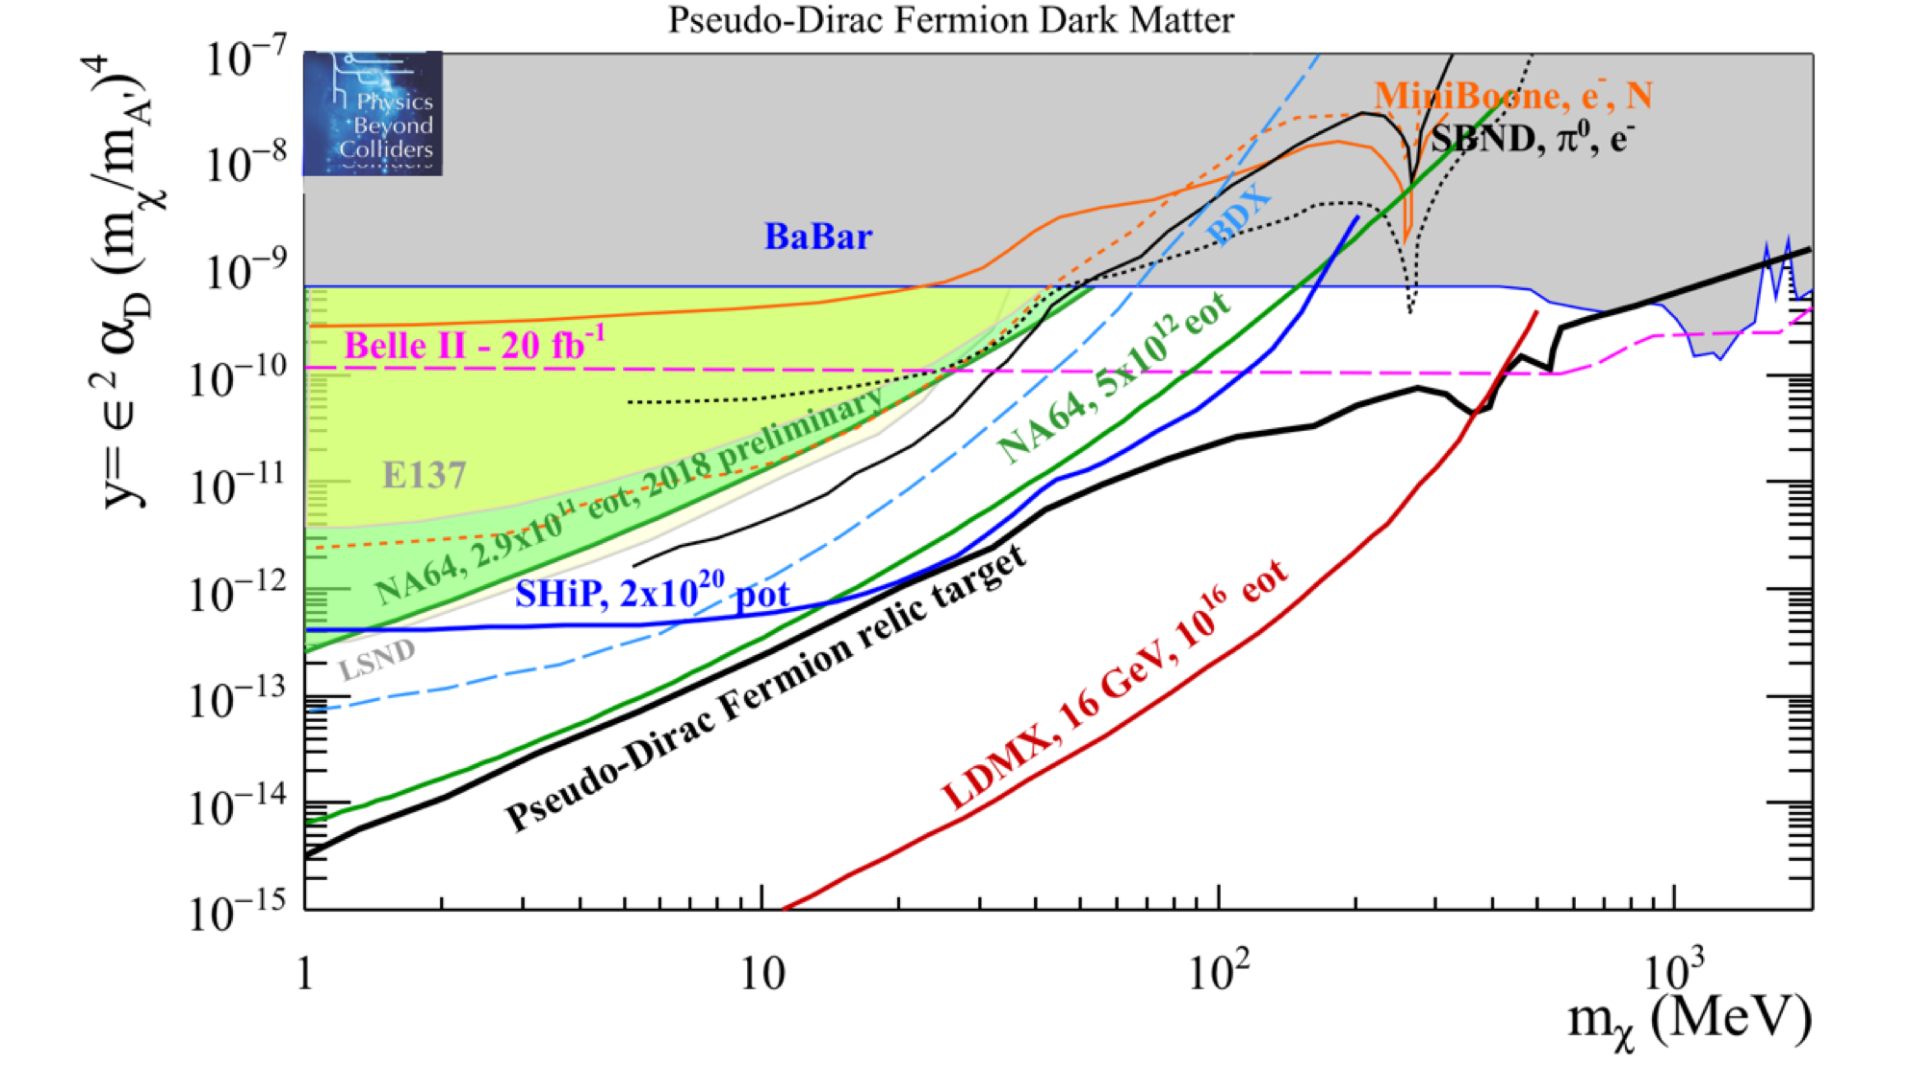
\includegraphics[width=\textwidth]{\pdirone/invisible-full-ps.png}
  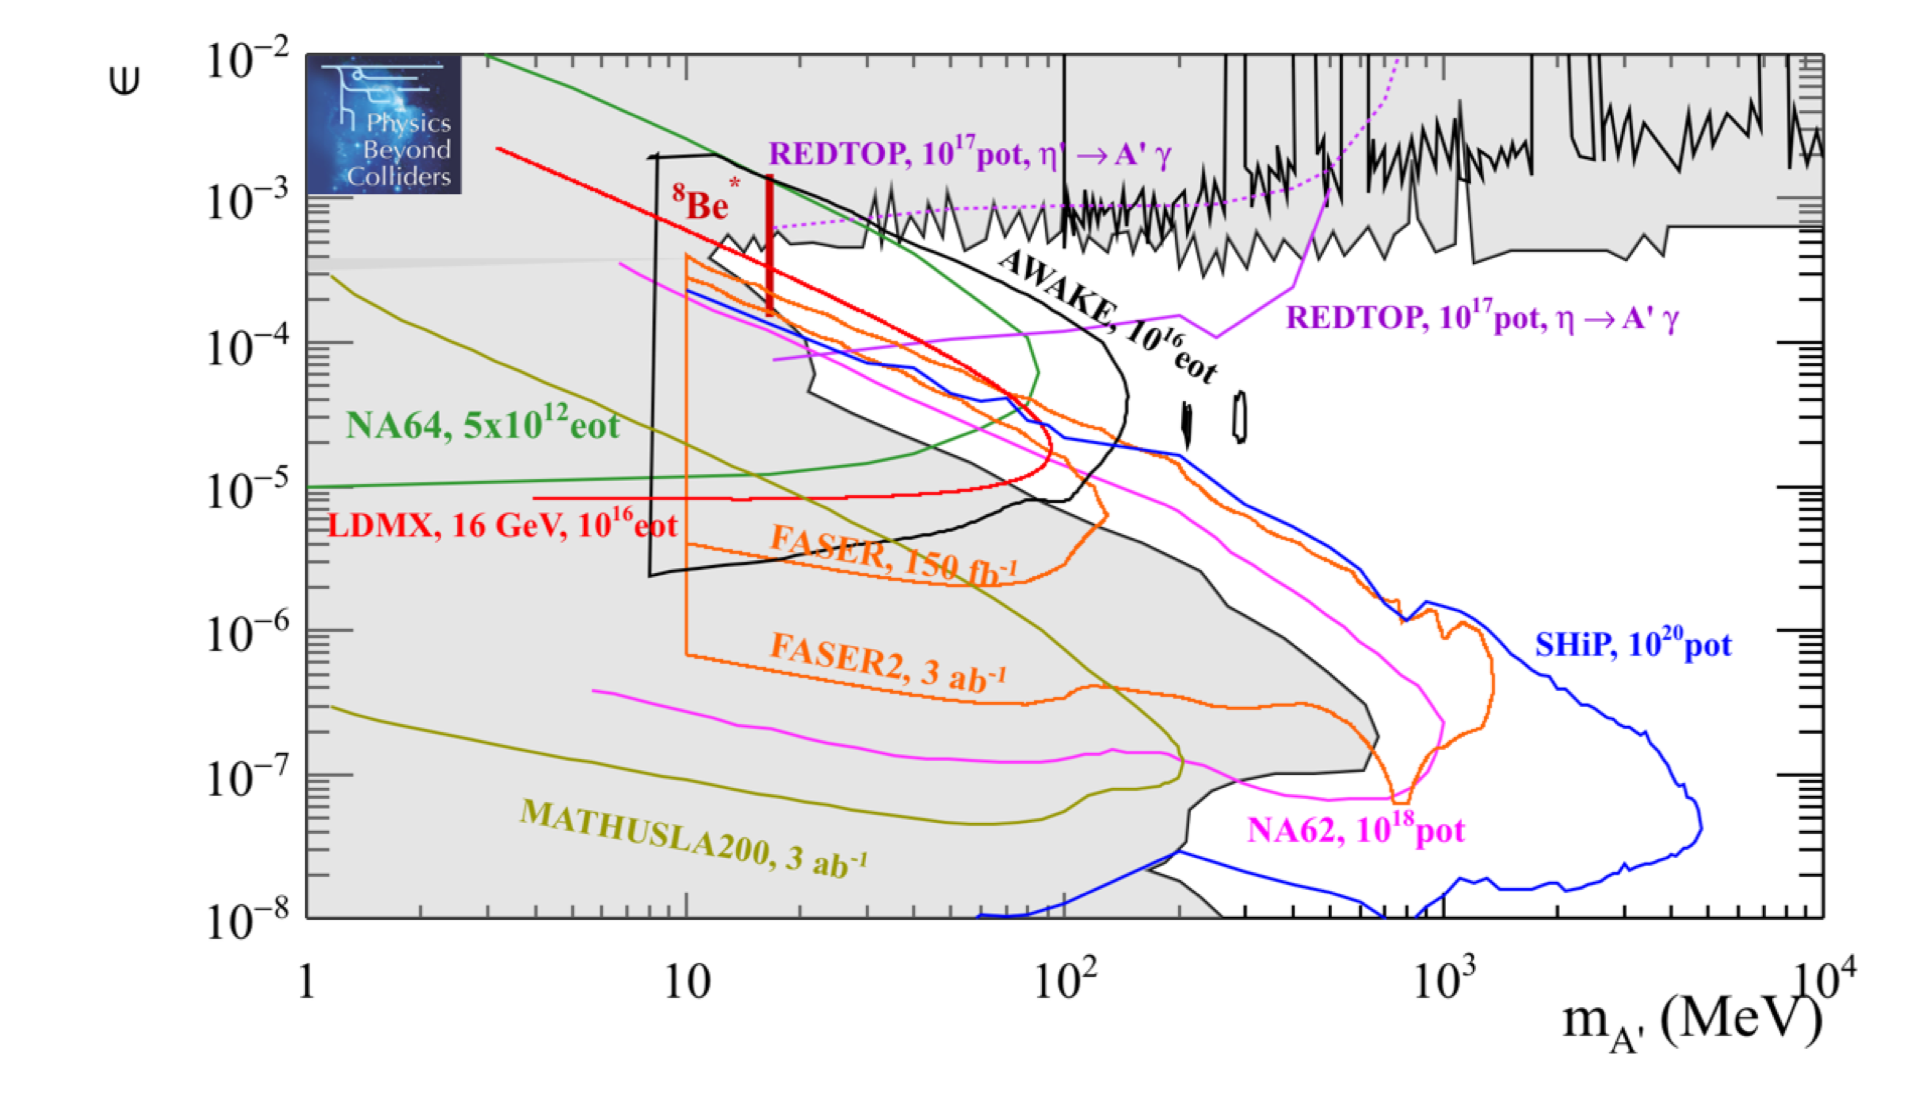
\includegraphics[width=\textwidth]{\pdirone/visible-full-ps.png}
  \caption[Current exclusion limit and project for Dark Photon in the physics community]{Current limits and expected sensitivities of experiments for dark photon mediators decay either to LDM particles (top) or SM particles (bottom). The top figures assumes $\alpha_d = 0.1$ and $m_{\DM}/m_{\chi} = 3$ \cite{pbc-book}.}
  \label{fig:dmplane-overview}
\end{figure}  

\section{The X17 anomaly}
\label{ch1:sec:dm-u1model-motivations-x17}

A big boost to search for the new light boson weakly coupled to Standard Model particles was caused by the recent observation of a 6.8$\sigma$ excess of events in the angular distribution of $\pair$ pairs produced in the nuclear transitions of the excited $^8$Be$^*$ nuclei to its ground state via IPC\footnote{Internal Pair Creation} of $\ee$ \cite{Krasznahorkay:2015iga}. The experiment used a proton beam to populate the isovector (17.6 \mev) and isoscalar state (18.15 \mev) 1$^+$ states in the $^8$ selectively using Lithium as initial target, and then detected the $\ee$ emitted in the reaction $^8$Be$^* \to ^8$Be using five plastic detector telescope in combination with position-sensitive MWPC\footnote{Multi-Wire Proportional Counters}. The concept of the experiment is depicted in Fig.\ref{fig:x17-setup}, and a precise description of the setup can be found in \cite{GULYAS201621}.

\begin{figure}[htb!]
  \centering
  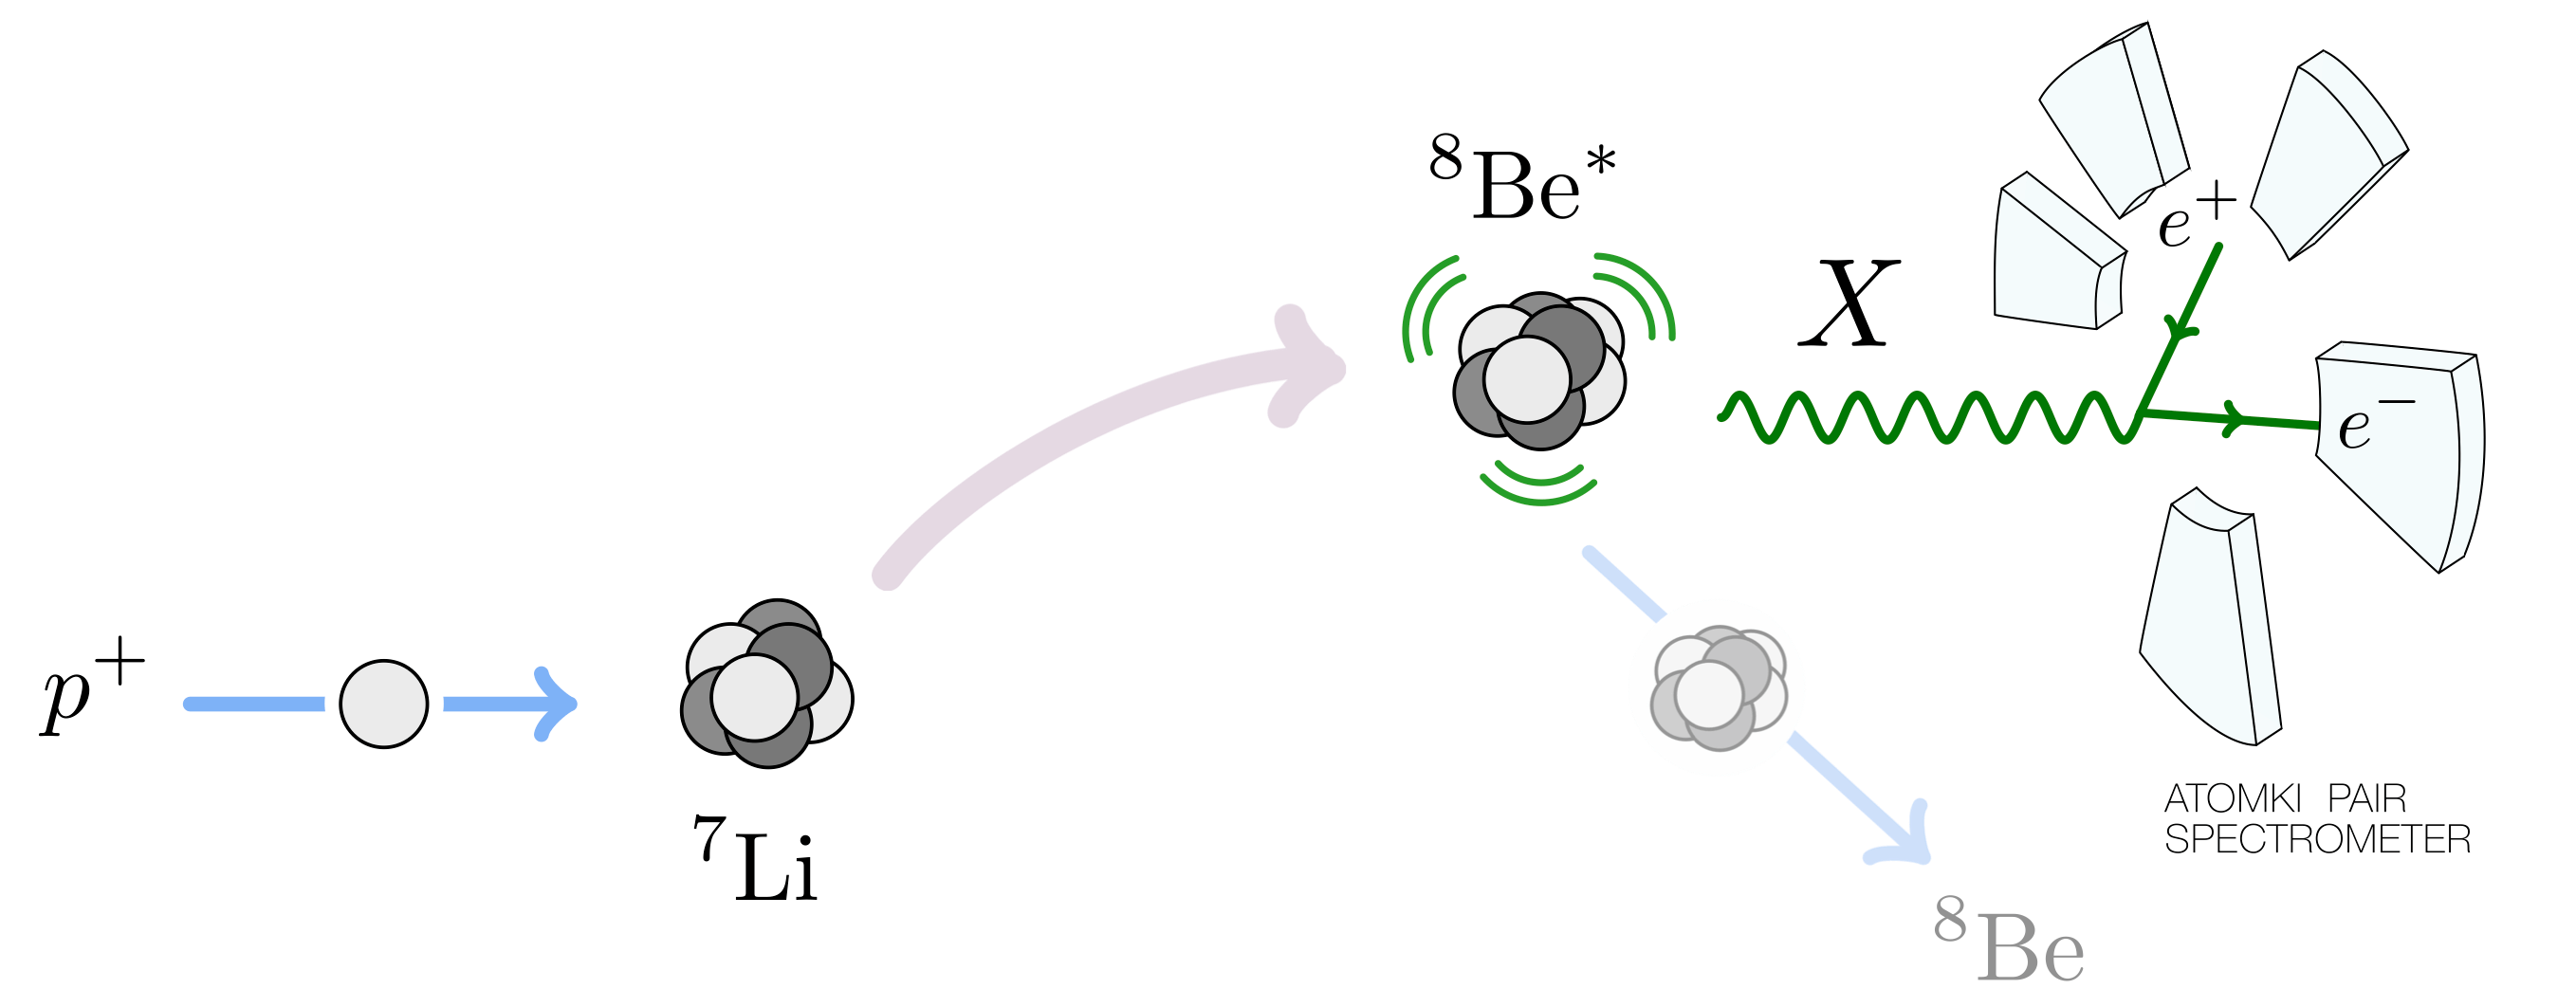
\includegraphics[width=\textwidth]{\pdirone/Atomki_setup.png}
  \caption[Sketch of the setup used to detect the $^8$Be anomaly.]{Sketch of the setup used to detect the $^8$Be anomaly. Lithium is bombarded by protons to excite the reaction $^7$Li$\to ^8$Be$^* \to ^8$Be. The aperture angle of the $\ee$ generate in the decay of the ground state is detected by a telescope made of five plastic scintillators. \cite{PhysRevD.95.035017}}
  \label{fig:x17-setup}
\end{figure}

While the spectrum of the isovector state showed good compatibility with the model, a substantial deviation was observed in the isoscalar state for angles $120 \si{\degree} < \theta_{\ee} < 160 \si{\degree}$. This deviation is challenging to explain in the context of nuclear physics \cite{Krasznahorkay:2015iga}, although some attempt can be found in \cite{Zhang:2017zap,Koch:2020ouk}. On the other hand, the anomaly can be easily interpreted as the emission of a gauge boson that mediates the $\ee$ pair at a specific energy. This hypothesis passes a good number of consistency checks. For example, since the mediator would be non-relativistic at these low energies, one would expect only $\ee$ pair with small asymmetry in energy to be effected. Indeed as shown in Fig.\ref{fig:be-anomaly}, this was verified to be true in the paper. The effect of mediator with different masses was modeled using MC-simulation, the best fit was found for $m_{\DMX} = 16.7 \pm 0.35^{\textrm{stat}} \pm 0.5^{\textrm{syst}}$ with an excellent compatibility of $\chi^2/\textrm{dof}$. Two years later, the same group investigated the anomaly using a new transition, the 21.01 \mev $0^- \to 0^+$ in the $^4$He atom. The setup was improved with an additional scintillator and the MWPC substituted with a more precise  DSSD array\footnote{Double-sided Silicon Strip Detector}. The results of this second experiment revealed a second anomaly, with a bump compatible with what previously measured, estimating a mass of $16.84 \pm 0.16^{\textrm{stat}} \pm 0.20^{\textrm{syst}}$ \cite{Krasznahorkay:2019lyl}. The result is even more striking considering the fact that the angular correlation differs for this transition, where the peak appeared in the region $110 \si{\degree} < \theta_{\ee} < 130 \si{\degree}$, which suggests that unknown systematics are not a viable explanation for this observation.

\begin{figure}[htb!]
  \centering
  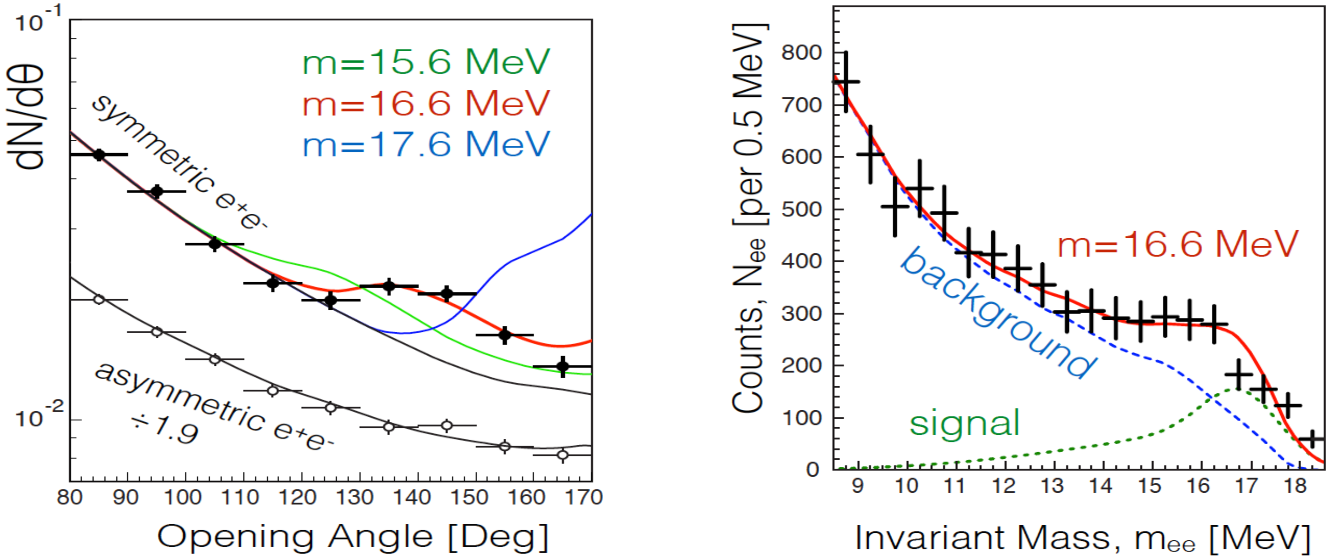
\includegraphics[width=\textwidth]{\pdirone/X17_spectrum.pdf}
  \caption[$^8$Be anomaly]{On the left: angular spectrum of the $\ee$ pair created in the reaction $^8$Be$^* \to ^8$Be of the isoscalar state of Beryllium into the ground state using proton energies $E_p$ = 1.10 \mev. The curve is presented for both asymmetric and symmetric pairs, with a rescale factor in the first case to separate the two curves. Simulations are shown for the expected spectrum (black lines) and the spectrum expected after adding a mediator of different masses (colored lines). On the right: same spectrum is plotted as invariant mass, best fit (red), background predicted (blue dotted), and signal measured (green dotted) are presented as well. \cite{Krasznahorkay:2015iga}}
  \label{fig:be-anomaly}
\end{figure}

Clearly, the experiment will need a separate confirmation by a different group as suggested in \cite{Feng:2020mbt}, but in the meantime, several models are being proposed to describe this unknown mediator responsible for the anomaly. A scalar candidate (a Dark Higgs) can't mediate the observed $^8$Be in the limit of conserved parity, which makes it not an ideal candidate \cite{PhysRevD.95.035017}. A pseudoscalar or ALP is likewise excluded if we consider only couplings to photons. The two main candidates not yet ruled out are the axial-vector and vector candidates, that we will explore here briefly. In this work, the focus will be on the vector candidate, that we will call $\DMX$ from now on. This is currently considered the most probable candidate for this anomaly, as the new result obtained for the $^4$He is well explained in this framework, while for the axial-vector case predicts a significant difference between decay widths of the two nuclei (factor $\sim10^2$) was expected but not observed \cite{Feng:2020mbt}. For completeness, we report here that other explanations were proposed to justify this anomaly in particle physics, see for example \cite{Nam:2019osu, Seto:2016pks}.

We might be tempted to use directly the model developed in Sec.\ref{ch1:sec:dm-u1model} in its visible channel incarnation. However, this is not possible, as this model is already well excluded by the $\pi^0 \to \DM \gamma$ searches by NA48/2 \cite{na48}. Other simple extensions to this model, like a mixing with the SM Z boson, or a light baryon-minus-lepton number (B - L) boson, are already constraint by several experiments \cite{PhysRevD.95.035017}. The current proposed solution is that the $\DMX$ disfavors coupling with protons. In mathematical terms, the relation $-0.067 < \epsilon_p/\epsilon_n < 0.078$ needs to be fulfilled to evade the current experimental limit, with the extreme scenario of $\epsilon_p = 0$ often taken as benchmark to study the phenomenology of this particle. This protophobic gauge vector boson might look a bit arbitrary, but an example of such a particle can be found in the well-known Z boson, which is protophobic at low energies \cite{PhysRevD.95.035017}. Recently, this model was criticized by pointing out that the production of $\DMX$ should be dominated by Dark Bremsstrahlung without going through any nuclear resonance for all proton beam energy above threshold, in direct contradiction with experimental observation \cite{zhang2020protophobic}.  However, in our experiment, the only assumption to be made is the existence of a coupling between $\DMX$ and the electron, which makes our sensitivity model-independent. This means our results can be easily extended to different models, like scalar, pseudo-scalar, and axial-vector boson. To cast the NA64 results, however, we will used the vector boson as benchmark model.

A precise discussion of the values permitted for each coupling is discussed in \cite{Feng:2016jff,PhysRevD.95.035017}, here we will limit the discussion on the limit imposed to $\epsilon_e$ \footnote{Effectively one can interpret $\epsilon_e = \epsilon$ and use the model developed in Sec.\ref{ch1:sec:dm-u1model}}. For a lower limit of the coupling $\epsilon$, we know that $\DMX$ needs to decay within the experimental setup to be detected by the telescope. This turns out to give a weaker bound ($\gtrsim 10^{-5}$) than what is provided by beam dump experiments such as SLAC E141 \cite{blum} of $\gtrsim 2 \times 10^{-4}$. For the upper limit, a coupling too strong would influence the good agreement between the experiment and the theory of the anomalous magnetic moment of the electron. By combining the two results, we obtain:

\begin{equation}
  \label{eq:x17-limits}
  2 \times 10^{-5} < \epsilon_e < 1.4 \times 10^{-3}
\end{equation}

Which translates to a lifetime (see Eq.\ref{eq:dm-decay-length}) of the order of $10^{-14}\lesssim \tau_X \lesssim 10^{-12}$~s.

Interestingly, such a new boson with a relatively large coupling to charged leptons could also resolve the tension between measured and predicted values of the $(g - 2)_{\mu}$. Another interesting result comes from the new measurement of $\alpha$ performed by Parker \textit{et al.} \cite{Parker191} which combined with the $(g-2)_e$ measurements result in a 2.4 $\sigma$ deviation from the QED predictions \cite{PhysRevLett.100.120801}. Should this tension be confirmed, the two constraints coming from the NA64 results and $(g - 2)_e$ would exclude the vector and axial-vector couplings explanation of $\DM$. On the other hand, models with nonzero V$\pm$A coupling constant with the electron would explain both electron and muon $(g - 2)$ anomalies \cite{Krasnikov:2019dgh}. In these models, the $\DM$ could have a coupling of $6.8\cdot 10^{-4} \lesssim \epsilon \lesssim 9.6 \cdot 10^{-4}$ which leaves an interesting region of the parameter space to be explored. These models motivated the study of the phenomenological aspects of such a light vector boson weakly coupled to quarks and leptons (see, e.g., Refs.~\cite{fayet1, fayet2, fayet3, fayet4,jk, cheng, Zhang:2017zap, ia, liang, bart}) and new experimental searches (see e.g., Refs.~\cite{battaglieri2017cosmic, nardi}).

Recently, the NA64 collaboration has reported new results that excluded the $\DM$ boson  with the coupling strength  to electrons in the range $1.2 \times 10^{-4} < \epsilon_e < 6.8 \times 10^{-4}$ \cite{Banerjee:2018vgk,Banerjee:2019hmi}, by using the calorimeter technique proposed in \cite{Gninenko:2013rka,Andreas:2013lya}. The remaining region of parameter space $6.8 \times 10^{-4} < \epsilon < 1.4 \times 10^{-3}$ is extremely challenging to probe in the current setup. The reason for this is the high coupling of this region that suppress exponentially the signal yield due to the low decay length. We can observe this by inverting Eq.\ref{eq:dm-rate-vis} and transform it into an expression to probe different value of $\epsilon$. If we define $\epsilon_{\textrm{up}}$ as the maximum $\epsilon$ that can be probed with a given set of data and we absorb all the constant in $C'$ we find:

\begin{equation}
  \label{eq:x17-coverage}
  \epsilon_{\textrm{up}} \sim C' \times \frac{E_0}{L_{\textrm{dump}}m^2_{\DMX}} \times \ln{\left(N_{EOT} \epsilon^2 \frac{m_e^2}{m_{\DMX}^2}\right)}
\end{equation}

Increasing the number of EOT only improves our limit logarithmically, and a quick computation shows that an unfeasible number $>10^{14}$ of events is needed to explore this region. On the other hand, changing the impact energy of the length of the dump improve our limit linearly. A new setup was proposed to increase the signal yield while keeping the background under control (and in principle even reduce it) by decreasing the length of the target. The new setup is described in Sec.\ref{ch5:sec:new-vismode-setup}, and was shown to be able to cover fully the remaining region.


%%% Local Variables:
%%% mode: latex
%%% TeX-master: "../PhDthesis"
%%% End:
